%Este trabalho está licenciado sob a Licença Creative Commons Atribuição-CompartilhaIgual 4.0 Internacional. Para ver uma cópia desta licença, visite https://creativecommons.org/licenses/by-sa/4.0/ ou envie uma carta para Creative Commons, PO Box 1866, Mountain View, CA 94042, USA.

\chapter{Conjuntos numéricos}
\index{Conjunto(s)!numéricos}
\section{Conjunto dos Números Naturais}

Os registros mais antigos de números encontrados por historiadores, são de símbolos que eram utilizados para registrar a quantidade de animais, estes símbolos foram sendo aprimorados com o desenvolvimento das sociedades e o aprimoramento da escrita, chegando ao sistema de numeração hindu-arábico que são os números como conhecemos hoje.

Estes símbolos que utilizamos para contar objetos são denominados números naturais ($\N$).\index{Números!naturais} O conjunto dos números naturais é composto por:
\[\N= \{0, 1, 2, 3, 4, 5, \ldots \},\]
e o conjunto dos números naturais sem o zero.
\[\N^{*}= \{1, 2, 3, 4, 5, \ldots \}.\]

Alguns historiadores acreditam que o zero foi o último deles a ser criado, justificando que no início não havia necessidade de registro no caso de não se ter posses. Ainda se discute dentro da matemática se o zero pertence ou não ao conjunto dos números naturais.

É importante notar que neste conjunto numérico estão bem definidas as operações de adição ($+$) e multiplicação ($\times$), mas não a subtração ($-$) e a divisão ($\div$).

\section{Conjunto dos Números Inteiros}

Com o surgimento do comércio, surge a necessidade dos comerciantes de registrarem a entrada e saída de bens em seus estabelecimentos, bem como seus lucros e suas despesas. Para efetuar estes registros eles criaram os números negativos,\index{Números!negativos} tendo assim como registrar posses usando números positivos\index{Números!positivos} e dívidas usando os números negativos.

Este conjunto de números negativos juntamente com os números naturais, forma o conjunto dos números inteiros ($\Z$):\index{Números!inteiros}
\[\Z= \{ \ldots , -5, -4, -3, -2, -1, 0, 1, 2, 3, 4, 5, \cdots \}\]

Observe que $\N \subset \Z$. E ainda que no conjunto dos números inteiros temos bem definidas as operações de soma ($+$) e subtração ($-$).

\section{Conjunto dos Números Racionais}

Note que no conjunto dos números inteiros ainda não é possível fazer todas as divisões, por exemplo $3 \div 2$ ainda não está definida, pois ainda não existe um número que represente este resultado. Para resolver este problema surge então o conjunto dos números racionais ($\Q$),\index{Números!racionais} que é formado por todos os números que podem ser escrito em forma de fração, ou seja o conjunto dos números que podem ser obtidos como resultado de alguma divisão, representamos este conjunto por:
\[\Q= \left\{ \frac{a}{b} \mid a, b \in \Z \text{ e } b \neq 0 \right\}.\]

Observe que $\N \subset \Z \subset \Q$. E ainda que no conjunto dos números racionais temos bem definidas as operações de soma ($+$), subtração ($-$), multiplicação/vezes ($\times$) e divisão/razão ($\div$). Porém as operações neste conjunto possuem algumas particularidades com as quais devemos ficar atentos, por isso iremos retomá-las na sequência de nossos estudos.

\subsection{Dízimas periódicas e não-periódicas}
As dízimas são números decimais com infinitas casas decimais, podendo haver alguma forma de repetição dos algarismos nas casas decimais, e neste caso a dízima é denominada periódica\index{Dízima!periódica} e é um número racional, ou não haver repetição alguma dos algarismos das casas decimais, neste caso a dízima é denominada não periódica\index{Dízima!não periódica} e é um número irracional. Estamos neste momento particularmente interessados nas dízimas periódicas.

 \vskip0.3cm
 \colorbox{azul}{
 \begin{minipage}{0.9\linewidth}
 \begin{center}
  Chamamos de \textbf{dízimas periódicas} os números decimais com infinitas casas decimais, nos quais a partir de alguma casa decimal, um algarismo ou um grupo de algarismos passa a se repetir infinitamente. O algarismo ou algarismos que se repetem infinitamente constituem o período da dízima.
 \end{center}
 \end{minipage}}
 \vskip0.3cm

 \begin{exem} Vejamos alguns exemplos de dízimas periódicas, e como dada a dízima encontrar a fração que a representa.

  \begin{enumerate}[a)]
   \item Considere o número $0,333 \ldots$, neste caso o período é $3$, assim,
   \[0,3333 \ldots= 0,\overline{3}= \frac{3}{9}= \frac{1}{3}\]
   De fato,
   \begin{eqnarray*}
    x &=& 0,3333 \ldots \\
    10x &=& 10 \ldots 0,3333 \ldots \\
    10x &=& 3,3333 \ldots \\
    10x &=& 3 + 0,3333 \ldots \\
    10x &=& 3 + x \\
    10x - x &=& 3 \\
    9x &=& 3 \\
    x &=& \frac{3}{9} \\
    0,3333 \ldots &=& \frac{1}{3}
   \end{eqnarray*}
   usando a mesma ideia conseguimos mostrar os exemplos abaixo.

   \item Considere o número $0,121212 \ldots$, neste caso o período é $12$, assim,
   \[0,121212 \ldots= 0,\overline{12}= \frac{12}{99}= \frac{4}{33}\]

   \item Considere o número $0,225225225 \ldots$, neste caso o período é $225$, assim,
   \[0,225225225 \ldots= 0,\overline{225}= \frac{225}{999}= \frac{75}{333}=\frac{25}{111}\]

   \item Considere o número $7,464646 \ldots$, neste caso o número tem uma parte inteira que é $7$ e uma parte decimal $0,464646 \ldots$ na qual o período é $46$. Portanto,
   \begin{eqnarray*}
    7,464646 \ldots &=& 7+0,464646 \ldots \\
    &=& 7 + \frac{46}{99} \\
    &=& \frac{7\cdot 99 + 46}{99}\\
    &=& \frac{739}{99}
   \end{eqnarray*}

   \item Considere o número $0,2\bar{5}= 0,2555 \ldots$, neste caso o período é $5$. Assim para obter a fração equivalente a esta dízima, procedemos da seguinte forma:
   \begin{eqnarray*}
    x &=& 0,2555 \ldots \\
    100x &=& 25,555 \ldots \\
    10x &=& 2,555 \ldots \\
    100x - 10x &=& 25,\bar{5} - 2, \bar{5} \\
    90x &=& 23 \\
    x&=& \frac{23}{90}
   \end{eqnarray*}

   \item Considere o número $1,317\bar{6}$, neste caso o período é $6$. Assim para obter a fração equivalente a esta dízima, procedemos da seguinte forma:
   \begin{eqnarray*}
    x &=& 1,317\bar{6} \\
    10000 x &=& 13176, \bar{6} \\
    1000 x &=& 1317,\bar{6}\\
    10000 x - 1000 x &=& 13176, \bar{6} - 1317,\bar{6}\\
    9000 x &=& 11859 \\
    x &=& \frac{11859}{9000}\\
    x &=& \frac{3953}{3000}
   \end{eqnarray*}

  \end{enumerate}

 \end{exem}

Com estes exemplos confirmamos que toda dízima periódica é um número racional, assim como os números inteiros, já que, se $a \in \Z$ então $a=\frac{a}{1}$, portanto $a \in \Q$, e os números com um número finito de casas decimais, por exemplo, $0,15= \frac{15}{100}$.


\section{Conjunto dos Números Irracionais}

Com o aprimoramento do cálculo de áreas, vem também a necessidade de sabendo a área, por exemplo do quadrado, descobrir quais as medidas de seus lados, dando então origem ao cálculo das raízes quadradas, surge portanto um novo problema, com os números criados até então nem todo número tem uma raiz quadrada. Para resolver este impasse, criou-se o conjunto dos números irracionais,\index{Números!irracionais} números estes que não podem ser representados por uma fração como por exemplo: $\sqrt{2}$, $\sqrt{3}$, $\sqrt{5}$, $\sqrt{7}$, pi ($\pi$), número de Euler ($e$), e muitos outros. Observe que $\Q \cap \I = \emptyset$.

Números decimais com infinitas casas decimais que não sejam dízimas periódicas são portanto exemplos de números irracionais.

\section{Conjunto dos Números Reais}

O conjunto dos números reais\index{Números!reais} nada mais é do que a união dos números racionais com os números irracionais, $\R= \Q \cup \I$, no qual as operações soma, subtração, multiplicação e divisão estão bem definidas.

\subsection{Relação de Ordem, Reta Real e o Valor Absoluto}

Do nosso dia-a-dia sabemos que como a matemática Wang Zhenyi nasceu em 1768 e a matemática Hertha Ayrton nasceu em 1854, então Wang é mais velha que Hertha, pois 1768 é anterior a 1854, ou podemos pensar também que 1768 é  menor que 1854, aqui estamos usando a relação de ordem\index{Ordem}\index{Desigualdades|see{Ordem}} dos números naturais para poder determinar quem nasceu primeiro e portanto é a mais velha, com esta relação de ordem das datas podemos construir uma cronologia dos acontecimentos históricos, que pode ser representada em uma reta cronológica.

Além dessa situação de datas podemos também pensar na questão das temperaturas, por exemplo temos que a maior temperatura registrada oficialmente no Brasil foi 44,7 °C em Bom Jesus, Piauí, em 21 de novembro de 2005, superando o recorde também oficial de Orleans, Santa Catarina, de 44,6 °C, de 6 de janeiro de 1963. E a menor temperatura registrada foi de –17,8 °C no Morro da Igreja, em Urubici, Santa Catarina, em 29 de junho de 1996 (registro extraoficial). A menor temperatura registrada oficialmente no país foi de –14,0 °C, no município de Caçador, no mesmo estado, em 11 de junho de 1952. Estas afirmações são possíveis pois sabemos que 44,7 é maior que 44,6 e -17,8 é menor que -14,0, para fazer estas comparações e decidir quando está mais frio e/ou mais quente estamos usando a relação de ordem dos números racionais.

Esta relação de ordem que usamos nos dois exemplos acima é apenas uma aplicação da relação de ordem que existe no conjunto dos números reais, que formalizamos da seguinte forma, dados os números $a, b \in \R$, dizemos que:

\begin{itemize}
\item $a$ é maior que $b$, ou $a > b$, se $(a - b)$ é um número positivo.
\item $a$ é maior ou igual a $b$, ou $a \geq b$, se $(a - b)$ é um número positivo ou zero.
\item $a$ é menor que $b$, ou $a < b$, se $(a - b)$ é um número negativo.
\item $a$ é menor ou igual a $b$, ou $a \leq b$, se $(a - b)$ é um número negativo ou zero.
\end{itemize}

Note que dizer que $a$ é menor que $b$ ($a < b$) é equivalente a dizer que $b$ é maior que $a$ ($b > a$), o que também usamos no nosso dia-a-dia sem maiores problemas.

O conjunto dos números reais é um exemplo de um conjunto totalmente ordenado, com a ordenação dada por ($\leq$) pois, quaisquer $x$, $y$, e $z \in \R$, satisfazem as seguintes condições:
\begin{itemize}
\item se $x \leq y$ e $y \leq x$ então $x= y$;
\item se $x \leq y$ e $y \leq z$ então $x \leq z$;
\item \textit{Tricotomia:} $x<y$ ou $x=y$ ou $x>y$.
\end{itemize}

Esta relação de ordem em $\R$ possui as seguintes propriedades.

\begin{prop} [Propriedades da relação de ordem]
\index{Ordem!propriedades da relação de}\index{Propriedades!da relação de ordem}
\label{prop.ordem} Dados $x, y, z \text{ e } w \in \R$ temos que:
\begin{enumerate}
\item Se $x \leq y$ e $z \leq w$ então $x+z \leq y+w$. De fato,
\[x+z \leq y+z \ \ \  \text{ e } \ \ \ y+z \leq y+w \Rightarrow x+z \leq y+w \ .\]
\item Se $0 \leq x \leq y$ e $0 \leq z \leq w$ então $0 \leq xz \leq yw$. De fato,
\[xz \leq yz \ \ \  \text{ e } \ \ \  zy \leq wy \Rightarrow xz \leq wy \ .\]
\item $x < y \Leftrightarrow x+z < y+z$;
\item $z>0 \Leftrightarrow z^{-1}>0$;
\item $z>0 \Leftrightarrow -z> 0$;
\item $z>0 \text{ e } x<y \Leftrightarrow xz<yz$;
\item $z<0 \text{ e } x<y \Leftrightarrow xz>yz$;
\item $0<x<y \Rightarrow 0< \dfrac{1}{y} < \dfrac{1}{x}$.
\end{enumerate}
\end{prop}

Este conceito de ordem dos números reais nos permite representá-los como pontos sobre uma reta orientada, chamada \textbf{reta real}\index{Reta real}, assim como representamos os anos em uma reta cronológica, e as temperaturas aparecem em ordem em um termômetro.

 \begin{figure}[H]
 \centering
 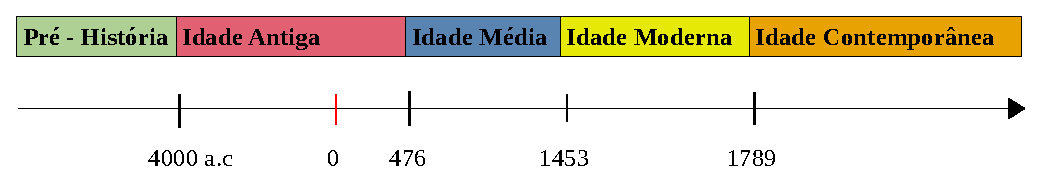
\includegraphics[width=15cm]{./cap_conjnum/figs/RetaCronologica}
 \caption{Linha do tempo história geral}
 \end{figure}

 \begin{figure}[H]
 \centering
 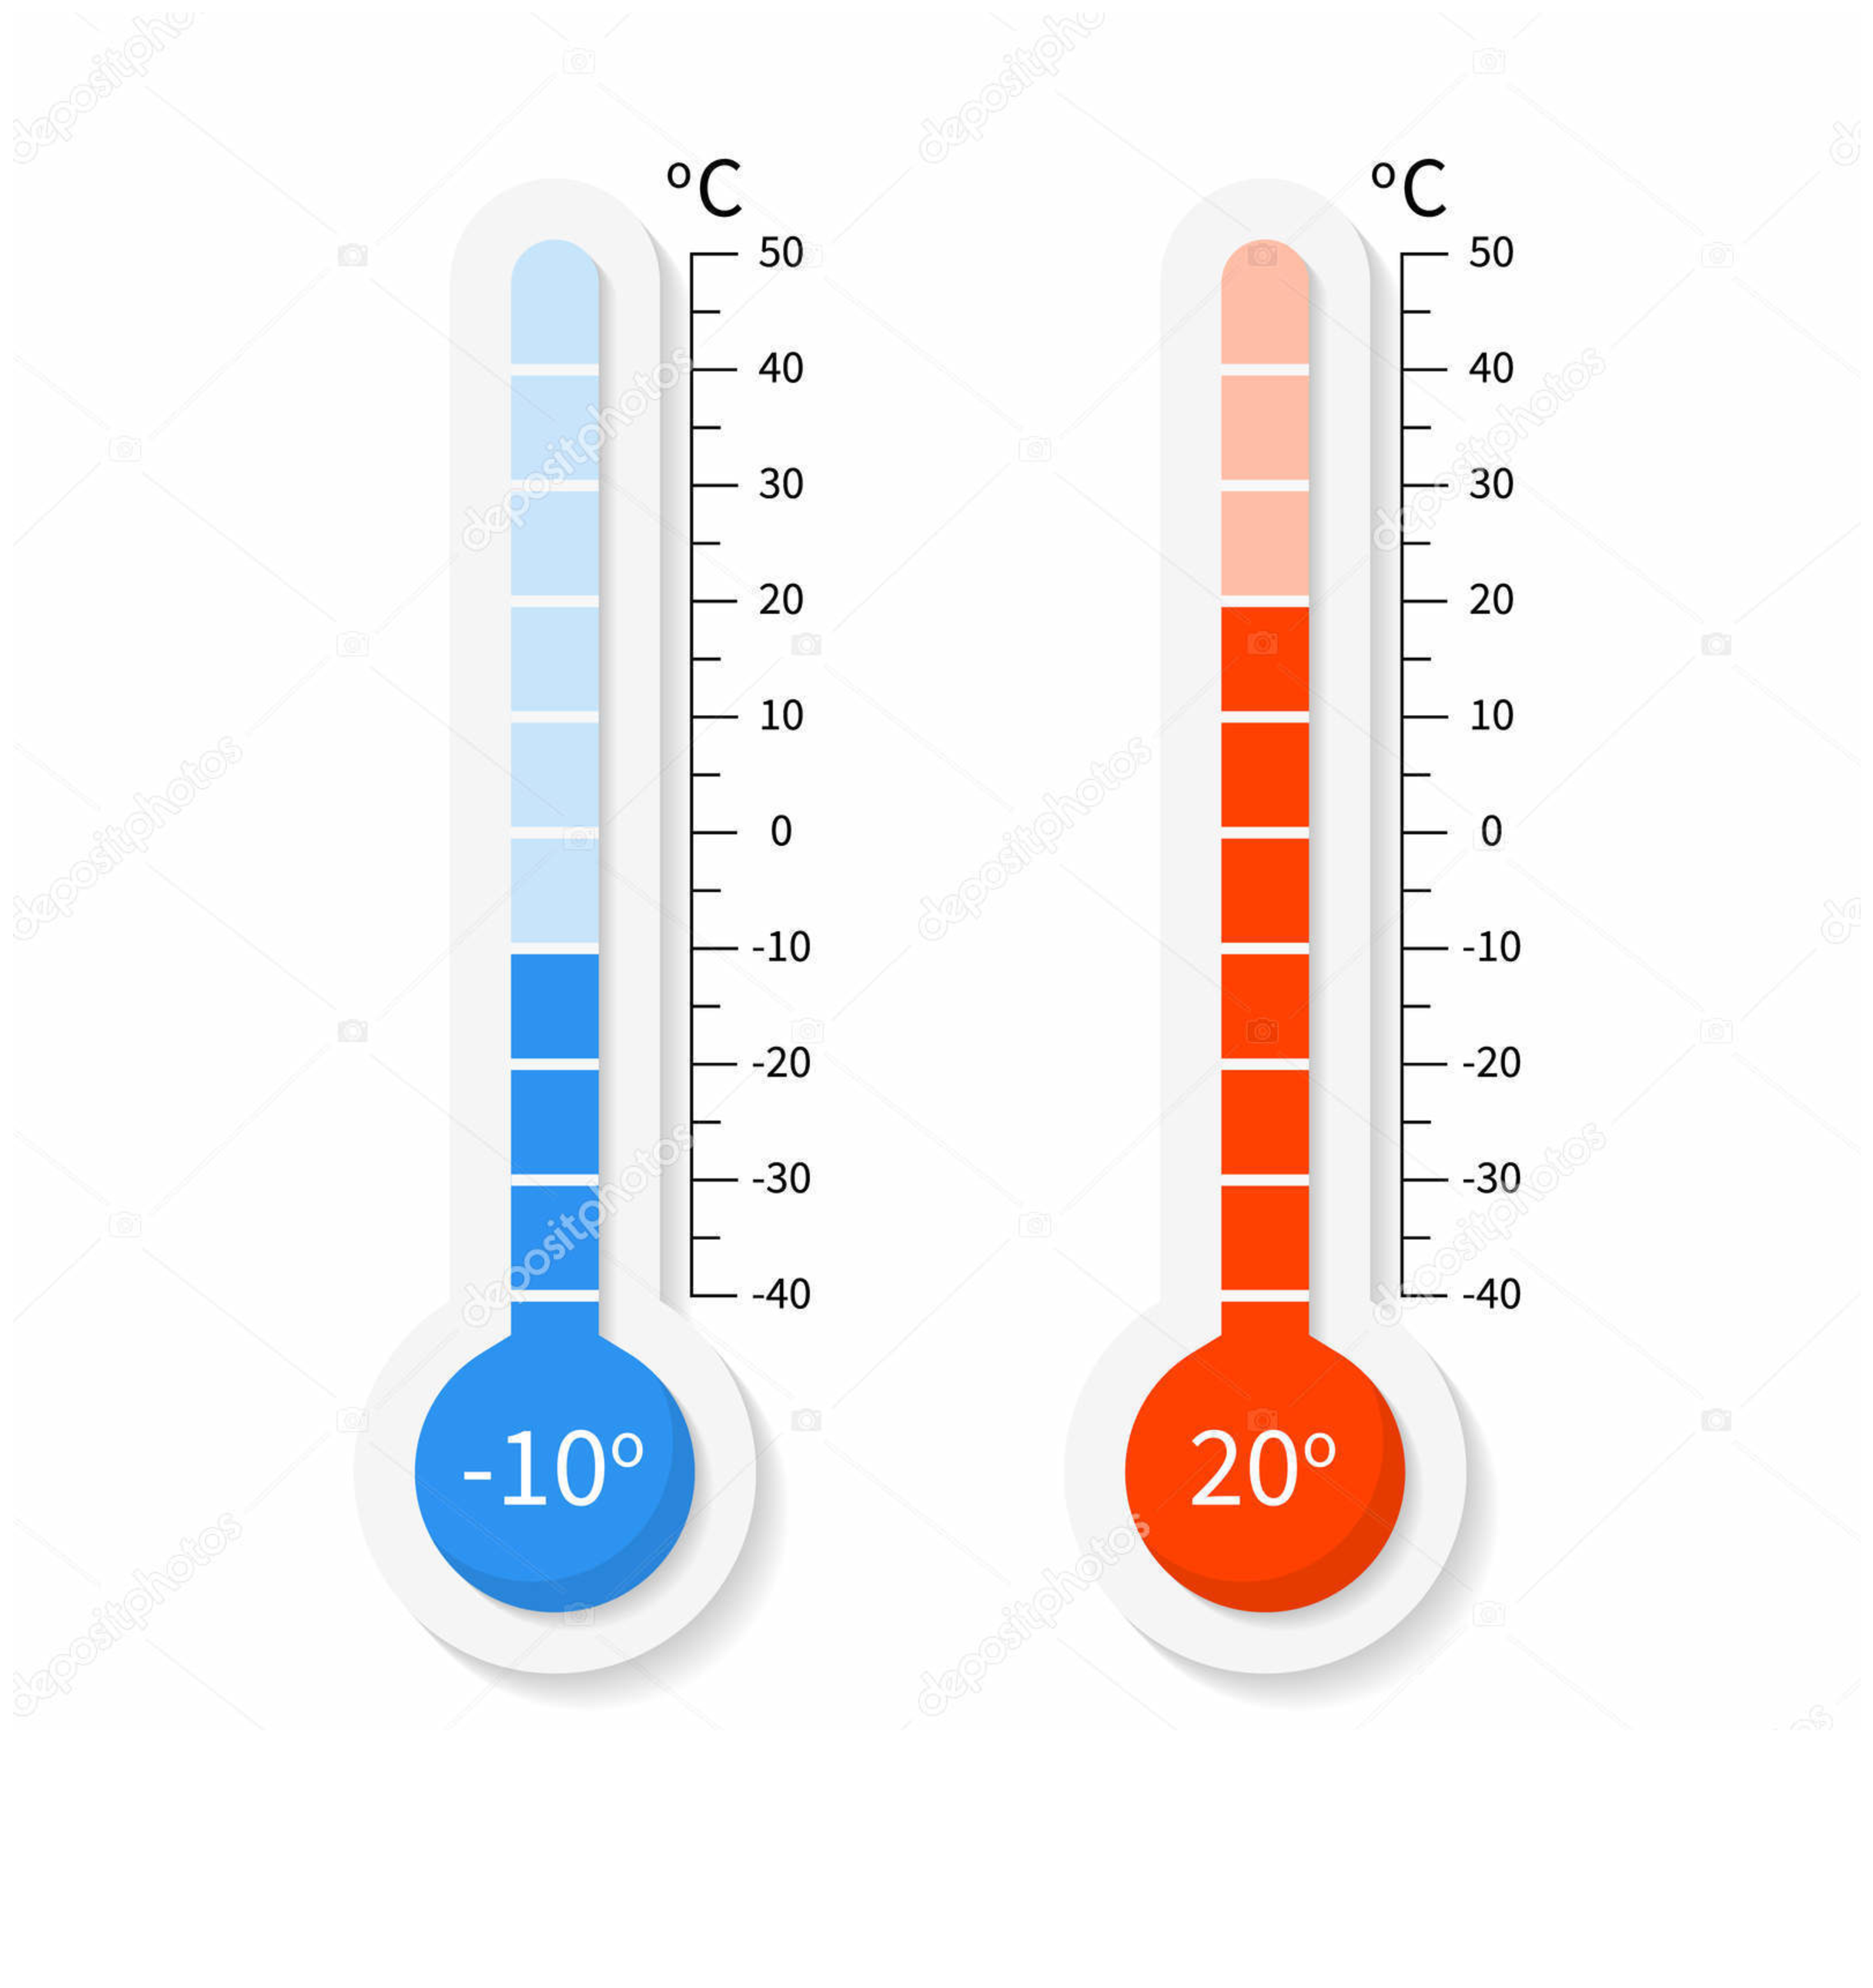
\includegraphics[width=6cm]{./cap_conjnum/figs/Termometro}
 \caption{Termômetros apresentando a temperatura em graus Celsius}
 \end{figure}

 Na reta real, o número $0$ (zero) serve como referência, sendo denominado origem. Os números positivos são representados à direita da origem e os números negativos à esquerda. Uma vez escolhida uma unidade de medida, exemplo centímetro, o número positivo $x$ é representado a exatamente $x$ unidade à direita do zero e o número $-x$ é representado a exatamente $x$ unidades à esquerda no zero.

  \begin{figure}[H]
 \centering
 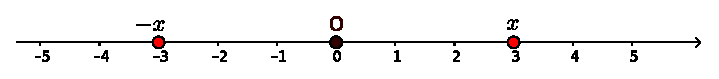
\includegraphics[width=15cm]{./cap_conjnum/figs/RetaReal}
 \caption{Reta Real}
 \end{figure}

 Na reta real da figura acima intuitivamente observarmos que a distância dos pontos $-x$ e $x$ até a origem (zero) é de exatamente três unidades, esta distância de um ponto $x$ da reta real à origem é denominada \textbf{valor absoluto}\index{Valor absoluto|see{Módulo}}\index{Módulo}, ou \textbf{módulo}, do número $x$, e é representada por $\abs{x}$. Assim, dizemos que:
\begin{itemize}
\item O valor absoluto de $-3$ é $3$, ou seja, $\abs{-3}= 3$;
\item O valor absoluto de $3$ é $3$, ou seja, $\abs{3}= 3$;
\end{itemize}
Generalizando esta ideia temos pela definição que:
\[
\abs{x}= \begin{cases}
      -x \ \ \text{se} \ \ x<0 \\
      x \ \ \text{se} \ \ x \geq 0 \ .
     \end{cases}
\]

O valor absoluto ou módulo de um número real conta com as seguintes propridades.

\begin{prop}[Propriedades do módulo]
 Para quaisquer $x, y \in \R$, são válidas as seguintes propriedades: \label{prop.modulo}
\begin{enumerate}
 \item $\abs{x} \geq 0$;
 \item $\abs{x}= 0 \Leftrightarrow x= 0$;
 \item $x \leq \abs{x}$;
 \item $-x \leq \abs{x}$;
 \item $\abs{-x}= \abs{x}$;
 \item $\abs{x}^2= x^2$, de fato,\\
 se $x \geq 0$, pela definição do módulo temos que $\abs{x}= x$ e daí $\abs{x}^2= x^2$, \\
 se $x < 0$, pela definição do módulo temos que $\abs{x}= -x$ e daí $\abs{x}^2=(-x)^2= x^2$.\\
 Portanto, para todo $x \in \R$, $\abs{x}^2= x^2$.

 \item $\abs{x^n}= \abs{x}^n$, se $n$ é par, de fato, \\
 se $x \geq 0$, pela definição do módulo temos que $\abs{x}= x$ e daí $\abs{x}^n= x^n$, \\
 se $x < 0$, pela definição do módulo temos que $\abs{x}= -x$ e daí $\abs{x}^n= (-x)^n= x^n$.\\
 Portanto, para todo $x \in \R$, $\abs{x}^n= x^n$.

 \item $\abs{x \cdot y}= \abs{x} \cdot \abs{y}$, de fato, \\
 \[\abs{x \cdot y}^2= (x \cdot y)^2= x^2 \cdot y^2= \abs{x}^2 \cdot \abs{y}^2= (\abs{x} \cdot \abs{y})^2 \ .\]
 Como $\abs{x \cdot y} \geqslant 0$ e $\abs{x} \cdot \abs{y} \geqslant 0$ resulta
 \[\abs{x \cdot y}= \abs{x} \cdot \abs{y} \ . \]

 \item $\abs{\dfrac{x}{y}}= \dfrac{\abs{x}}{\abs{y}}$, para $y \neq 0$, de fato, \\
 \[\abs{\dfrac{x}{y}}^2= \left(\dfrac{x}{y} \right)^2= \dfrac{x^2}{y^2}= \dfrac{\abs{x}^2}{\abs{y}^2}= \left( \dfrac{\abs{x}}{\abs{y}} \right)^2 \ . \]
 Como $\abs{\dfrac{x}{y}} \geq 0$ e $\dfrac{\abs{x}}{\abs{y}} \geq 0$ resulta que
 \[\abs{\dfrac{x}{y}}= \dfrac{\abs{x}}{\abs{y}} \ .\]

 \item Desigualdade triangular: $\abs{x+y}\leq \abs{x}+\abs{y}$, de fato, \\
 se $x + y \geqslant 0$, pela definição de módulo, $\abs{x+y}= x+y \leq \abs{x} + \abs{y}$; \\
 se $x + y < 0$, pela definição de módulo, $\abs{x+y}= -(x+y)= -x-y \leq \abs{x} + \abs{y}$. \\
 Logo, para quaisquer $x, y \in \R$ temos que
 \[\abs{x+y} \leq \abs{x}+\abs{y} \ .\]

 \item $\abs{x-y} \leq \abs{x} + \abs{y}$, de fato \\
 Note que $x-y= x+ (-y)$, logo $\abs{x-y}= \abs{x+ (-y)}$ aplicando a desigualdade trinagular temos,
 \[\abs{x-y}= \abs{x+ (-y)} \leq \abs{x} + \abs{-y}= \abs{x} + \abs{y} \ .\]

 \item $\abs{\abs{x} - \abs{y}} \leq \abs{x - y}$, para mostrar esta desigualdade vamos fazer por partes.
 \begin{itemize}
 \item $\abs{x} - \abs{y} \leq \abs{x - y}$, \\
 de fato, pela desigualdade triangular temos que
 \[\abs{z+y} \leq \abs{z} + \abs{y}\]
 subtraíndo $\abs{y}$ a ambos os termos temos,
 \[\abs{z+y} - \abs{y} \leq \abs{z}\]
 fazendo $x= z+y$ temos que $z=x-y$ substituindo estes valores na equação acima obtemos
 \[\abs{x} - \abs{y} \leq \abs{x-y} \ . \]
 \item $\abs{y} - \abs{x} \leq \abs{x - y}$, \\
 de fato, pela desigualdade triangular temos que
 \[\abs{x+z} \leq \abs{x} + \abs{z}\]
 subtraíndo $\abs{x}$ a ambos os termos temos,
 \[\abs{x+z} - \abs{x} \leq \abs{z}\]
 fazendo $y= x+z$ temos que $z=y-x$ substituindo estes valores na equação acima obtemos
 \[\abs{y} - \abs{x} \leq \abs{y-x}= \abs{x-y} \ . \]
 \end{itemize}

 Portanto,
 \[ \abs{\abs{x} - \abs{y}} = \pm (\abs{x} - \abs{y}) \leq \abs{x-y} \ .\]

\end{enumerate}
\end{prop}




Apesar de nossos estudos neste curso ser focado no conjunto dos números reais, neste conjunto numérico não conseguimos resolver todos os problemas matemáticos, em virtude disso, temos por exemplo o conjunto do números complexos, quatérnios, entre outros, desses mais avançados vamos falar um pouquinho dos números complexos pois neste conjunto é possível calcular raíz quadrada de qualquer número, o que não ocorre nos reais.

\section{Conjunto dos números Complexos}

Para resolver o problema da raiz quadrada de um número negativo, criou-se o número imaginário puro $i$, definido por $\iu= \sqrt{-1}$, portanto $\iu^2= -1$, criou-se assim um número $\iu$ que elevado ao quadrado desse $-1$. Temos agora como calcular a raiz quadrada de qualquer número real. Definimos a partir deste número imaginário o conjunto dos números complexos por:
\[\C= \{a + b\iu \mid a, b \in \R \} ,\]
cujas operações apresentam algumas particularidades e portanto trataremos delas mais adiante.

Note que, se tivermos $b=0$, estamos com o conjunto dos números reais, portanto $\R \subset \C$. Para fixar a ordem de continência destes conjuntos numéricos, observemos o diagrama de Venn abaixo.

 \begin{figure}[H]
 \centering
    \fbox{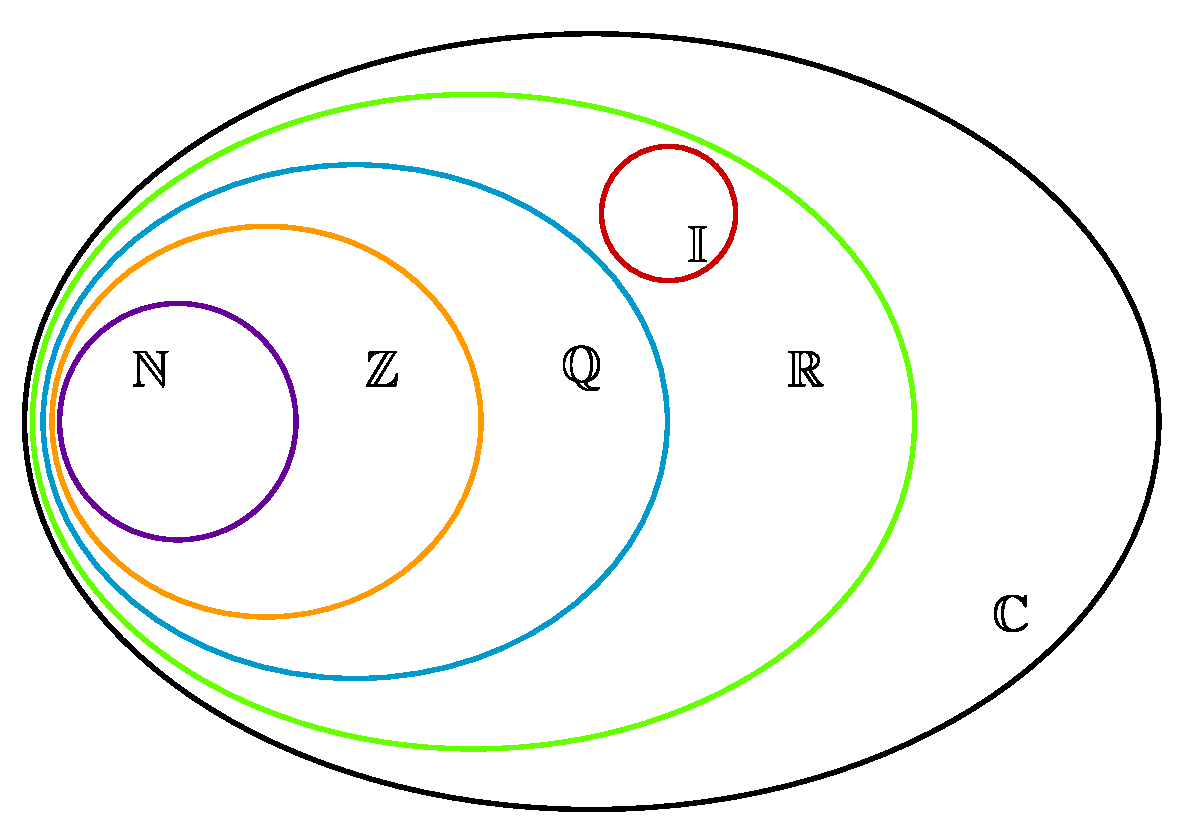
\includegraphics[width=7.5cm]{./cap_conjnum/figs/diagrama_conjuntos}}
    \caption{Representação conjuntos numéricos}
  \end{figure}

\section{Subconjuntos numéricos e suas representações}

\textbf{Intervalos numéricos limitados}\index{Intervalos numéricos!limitados}
\begin{itemize}
 \item Intervalo aberto: $]a, b[= \{x \in \R \mid a < x < b\}$;
 \begin{figure}[H]
 \centering
 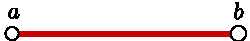
\includegraphics[width=3.5cm]{./cap_conjnum/figs/aberto-a-aberto-b}
 \end{figure}
 \item Intervalo fechado: $[a, b]= \{x \in \R \mid a \leq x \leq b\}$;
 \begin{figure}[H]
 \centering
 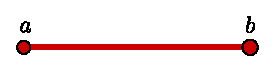
\includegraphics[width=3.5cm]{./cap_conjnum/figs/fechado-a-fechado-b}
 \end{figure}
 \item Intervalo aberto à direita e fechado à esquerda: $[a, b[= \{x \in \R \mid a \leq x < b\}$;
 \begin{figure}[H]
 \centering
 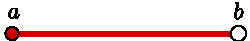
\includegraphics[width=3.5cm]{./cap_conjnum/figs/fechado-a-aberto-b}
 \end{figure}
 \item Intervalo aberto à esquerda e fechado à direita: $]a, b]= \{x \in \R \mid a < x \leq b\}$.
 \begin{figure}[H]
 \centering
 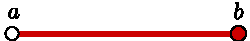
\includegraphics[width=3.5cm]{./cap_conjnum/figs/aberto-a-fechado-b}
 \end{figure}
\end{itemize}



\textbf{Intervalos numéricos ilimitados}\index{Intervalos numéricos!ilimitados}
\begin{itemize}
\item Conjunto dos números reais maiores que $a$: $[a, +\infty[ = \{ x \in \R \mid a < x \}$
 \begin{figure}[H]
 \centering
 
\includegraphics[width=3.5cm]{./cap_conjnum/figs/aberto-a-inf}
 \end{figure}

\item Conjunto dos números reais maiores ou iguais à $a$: $[a, +\infty[ = \{ x \in \R \mid a \leq x \}$
 \begin{figure}[H]
 \centering
 
\includegraphics[width=3.5cm]{./cap_conjnum/figs/fechado-a-inf}
 \end{figure}

\item Conjunto dos números reais menores que $b$: $]-\infty, b] = \{ x \in \R \mid x < b \}$
 \begin{figure}[H]
 \centering
 
\includegraphics[width=3.5cm]{./cap_conjnum/figs/inf-aberto-b}
 \end{figure}

\item Conjunto dos números reais menores ou iguais à $b$: $]-\infty, b] = \{ x \in \R \mid x \leq b \}$
 \begin{figure}[H]
 \centering
 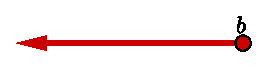
\includegraphics[width=3.5cm]{./cap_conjnum/figs/inf-fechado-b}
 \end{figure}

\item Conjunto dos números reais: $]-\infty, +\infty[ = \R$
 \begin{figure}[H]
 \centering
 
\includegraphics[width=7.5cm]{./cap_conjnum/figs/reta}
 \end{figure}
\end{itemize}


\textbf{Outros subconjuntos dos números reais}
\begin{itemize}
 \item Conjunto dos números reais não-nulos: $\R^{*}=\{x \in \R \mid x \neq 0\}$;
 \begin{figure}[H]
 \centering
 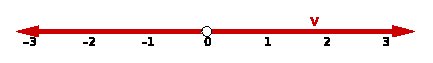
\includegraphics[width=7.5cm]{./cap_conjnum/figs/n-nulos}
 \end{figure}
 \item Conjunto dos números reais não-negativos: $\R_{+}=\{x \in \R \mid x \geq 0\}$;
 \begin{figure}[H]
 \centering
 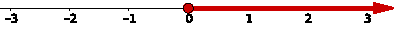
\includegraphics[width=7.5cm]{./cap_conjnum/figs/n-negativos}
 \end{figure}
 \item Conjunto dos números reais positivos: $\R^{*}_{+}=\{x \in \R \mid x > 0\}$;
 \begin{figure}[H]
 \centering
 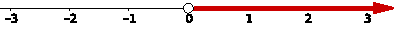
\includegraphics[width=7.5cm]{./cap_conjnum/figs/positivos}
 \end{figure}
 \item Conjunto dos números reais não-positivos: $\R_{-}=\{x \in \R \mid x \leq 0\}$;
 \begin{figure}[H]
 \centering
 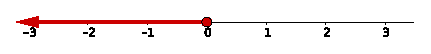
\includegraphics[width=7.5cm]{./cap_conjnum/figs/n-positivos}
 \end{figure}
 \item Conjunto dos números reais negativos: $\R^{*}_{-}=\{x \in \R \mid x < 0\}$.
 \begin{figure}[H]
 \centering
 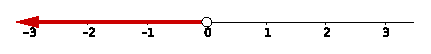
\includegraphics[width=7.5cm]{./cap_conjnum/figs/negativos}
 \end{figure}
\end{itemize}

\section{Operações com conjuntos numéricos}

Vamos agora apresentar alguns exemplos de como aplicar as operações de união, interseção, diferença e produto cartesiano entre conjuntos no contexto de subconjuntos dos números reais. A atenção especial a este tipo de conjunto se deve a extensa utilização destas operações para determinar o conjunto solução de equação e inequações, bem como para determinar o domínio de algumas funções, temas centrais deste curso.

\begin{itemize}
 \item Caso $a< b< c< d$ temos que $[a, b] \cup [c, d]$ pode ser representado por:
  \begin{figure}[H]
 \centering
 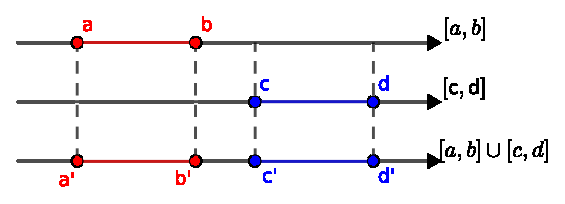
\includegraphics[width=8cm]{./cap_conjnum/figs/uniaoabcd}
 \end{figure}

 \item Caso $a< c< b< d$ temos que $[a, b] \cup [c, d]= [a, d]$ pode ser representado por:
  \begin{figure}[H]
 \centering
 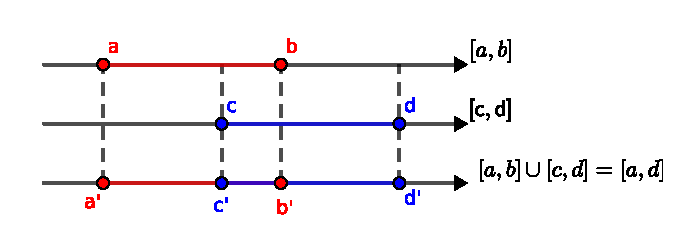
\includegraphics[width=8cm]{./cap_conjnum/figs/uniaoacbd}
 \end{figure}

  \item Caso $a< c< d< b$ temos que $[a, b] \cup [c, d]= [a, b]$ pode ser representado por:
  \begin{figure}[H]
 \centering
 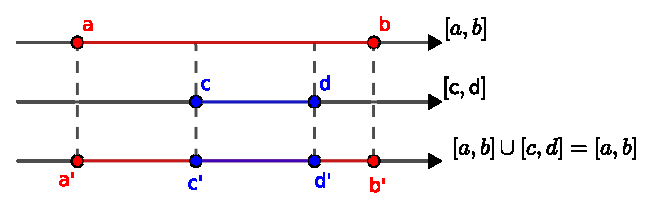
\includegraphics[width=8cm]{./cap_conjnum/figs/uniaoacdb}
 \end{figure}

 \item Caso $a< b< c< d$ temos que $]a, b[ \cup ]c, d[$ pode ser representado por:
  \begin{figure}[H]
 \centering
 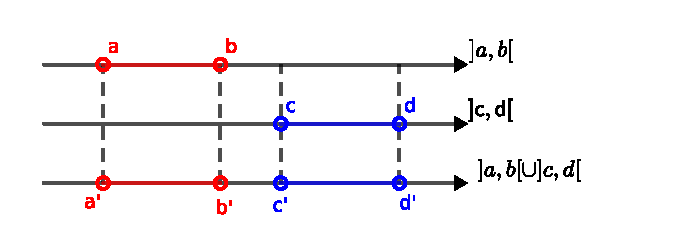
\includegraphics[width=8cm]{./cap_conjnum/figs/uniao-a-b-c-d}
 \end{figure}

 \item Caso $a< c< b< d$ temos que $]a, b[ \cup ]c, d[= ]a, d[$ pode ser representado por:
  \begin{figure}[H]
 \centering
 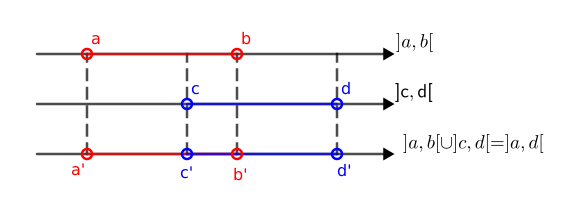
\includegraphics[width=8cm]{./cap_conjnum/figs/uniao-acb-d}
 \end{figure}

   \item Caso $a< c< d< b$ temos que $]a, b[ \cup ]c, d[= ]a, b[$ pode ser representado por:
  \begin{figure}[H]
 \centering
 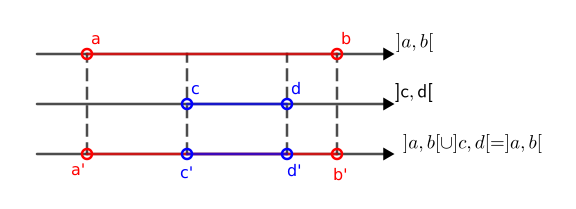
\includegraphics[width=8cm]{./cap_conjnum/figs/uniao-acd-b}
 \end{figure}

 %%%%%%%%%%%%%%%%%%%%
 \item Caso $a< b< c< d$ temos que $[a, b] \cap [c, d]= \emptyset$ pode ser representado por:
  \begin{figure}[H]
 \centering
 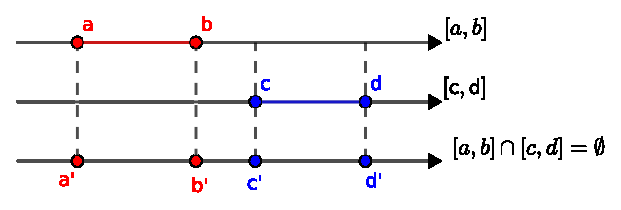
\includegraphics[width=8cm]{./cap_conjnum/figs/intersecaoabcd}
 \end{figure}

 \item Caso $a< c< b< d$ temos que $[a, b] \cap [c, d]= [c, b]$ pode ser representado por:
  \begin{figure}[H]
 \centering
 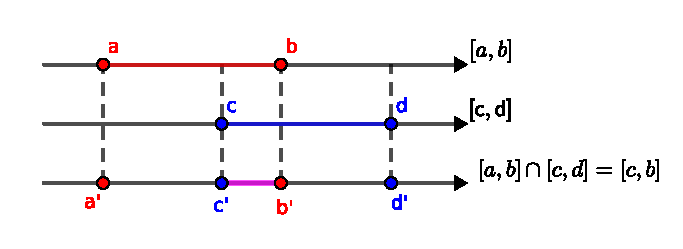
\includegraphics[width=8cm]{./cap_conjnum/figs/intersecaoacbd}
 \end{figure}

  \item Caso $a< c< d< b$ temos que $[a, b] \cap [c, d]= [c, d]$ pode ser representado por:
  \begin{figure}[H]
 \centering
 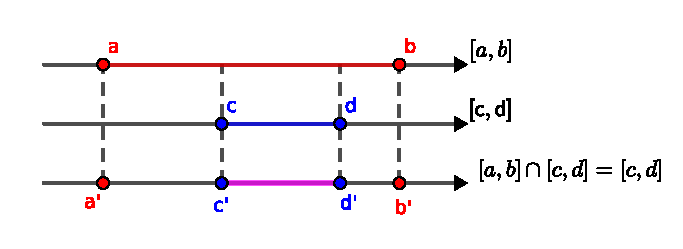
\includegraphics[width=8cm]{./cap_conjnum/figs/intersecaoacdb}
 \end{figure}

 \item Caso $a< b< c< d$ temos que $]a, b[ \cap ]c, d[ = \emptyset$ pode ser representado por:
  \begin{figure}[H]
 \centering
 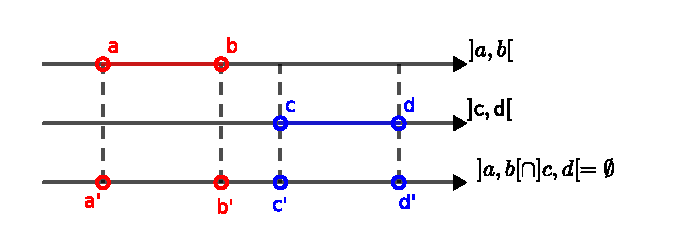
\includegraphics[width=8cm]{./cap_conjnum/figs/intersecao-a-b-c-d}
 \end{figure}

 \item Caso $a< c< b< d$ temos que $]a, b[ \cap ]c, d[= ]c, b[$ pode ser representado por:
  \begin{figure}[H]
 \centering
 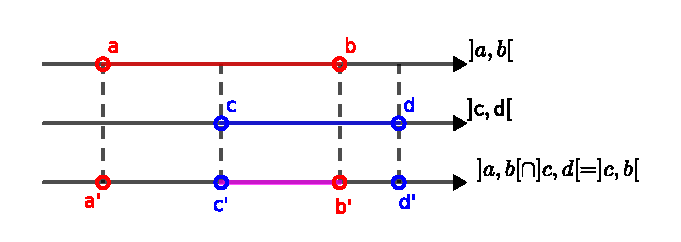
\includegraphics[width=8cm]{./cap_conjnum/figs/intersecaoa-c-bd}
 \end{figure}

   \item Caso $a< c< d< b$ temos que $]a, b[ \cap ]c, d[= ]c, d[$ pode ser representado por:
  \begin{figure}[H]
 \centering
 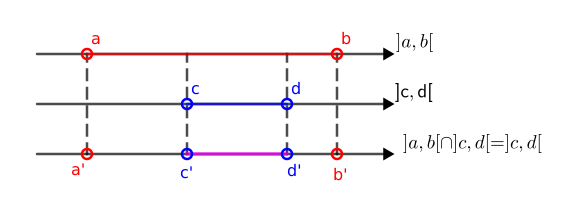
\includegraphics[width=8cm]{./cap_conjnum/figs/intersecaoa-c-db}
 \end{figure}

 \item Considere agora o conjunto $A= [1, \infty[ \times [2, 4[$, que é também representado da seguinte forma:
 \[A= \{(x, y) \in \R^2 \mid 1 \leq x \text{ e } 2 \leq y < 4 \}\]
   \begin{figure}[H]
 \centering
 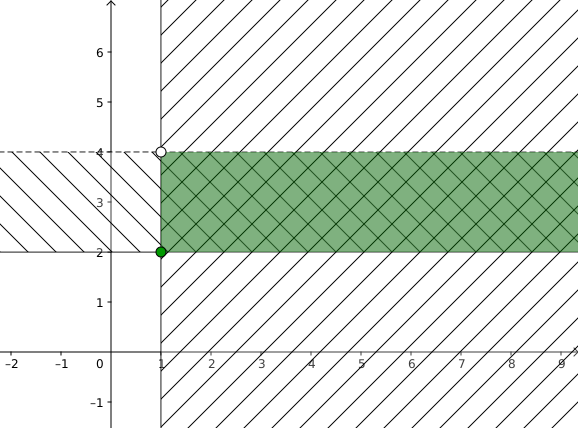
\includegraphics[width=8cm]{./cap_conjnum/figs/cartesiano1infty24}
 \end{figure}

 \item Considere agora o conjunto $B= [1, 4[ \times [3, 5[$, que é também representado da seguinte forma:
 \[B= \{(x, y) \in \R^2 \mid 1 \leq x \leq 4 \text{ e } 3 \leq y < 5 \}\]
   \begin{figure}[H]
 \centering
 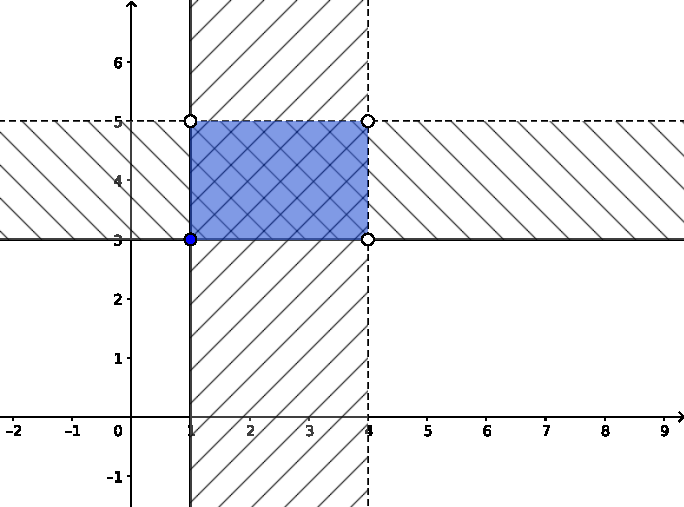
\includegraphics[width=8cm]{./cap_conjnum/figs/cartesiano1435}
 \end{figure}

 \item Considerando agora os seguintes conjuntos $A$ e $B$:
 \[A= \{(x, y) \in \R^2 \mid 1 \leq x \text{ e } 2 \leq y < 4 \}\]
 \[B= \{(x, y) \in \R^2 \mid 1 \leq x \leq 4 \text{ e } 3 \leq y < 5 \}\]
 temos que:

 \item $A \cap B$ é representado graficamente por:
    \begin{figure}[H]
 \centering
 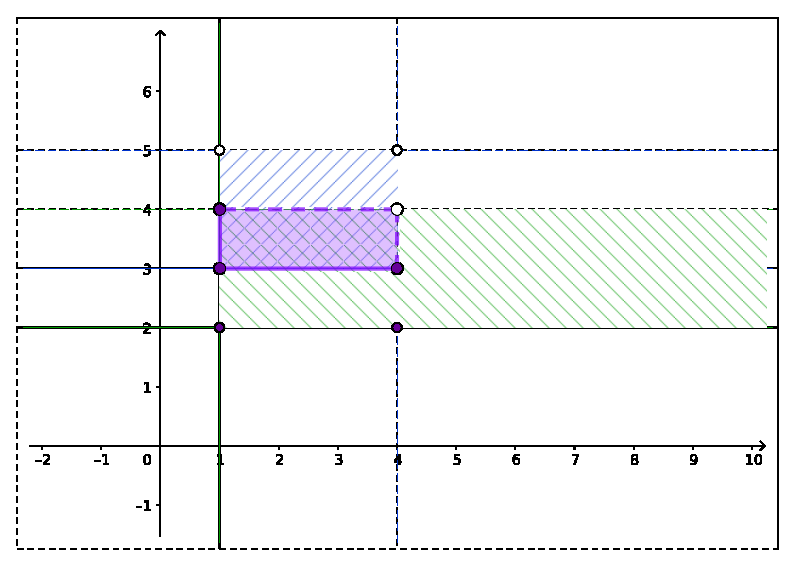
\includegraphics[width=8cm]{./cap_conjnum/figs/cartesianointersecao}
 \end{figure}

 \begin{itemize}
 \item $A \cup B$ é representado graficamente por:
    \begin{figure}[H]
 \centering
 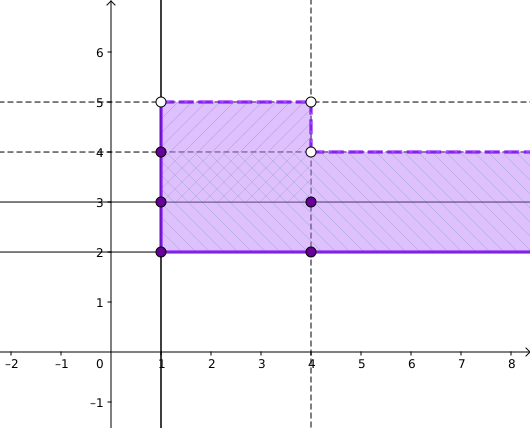
\includegraphics[width=8cm]{./cap_conjnum/figs/cartesianouniao}
 \end{figure}

 \end{itemize}

\end{itemize}

\section{Exercícios}

\begin{exer}
(FUNDATEC - 2012)  Considerando os seguintes conjuntos:
         \[ A = \{x \in \N \mid x < 5\}\]
         \[ B = \{x \in \Z \mid 3x + 4 = 13\}\]
         \[ C = \{x \in \R \mid x^2 + x - 12 = 0 \} \]
   é correto afirmar que:
   \begin{enumerate}
   \item $A \cap B = \{ 1,2,3\}$
   \item $A \cup B = B$
   \item $A - B = \{0,1,2,4\}$
   \item $A \cup B \subset C$
   \item $B \cup C= \R$
  \end{enumerate}
\end{exer}

\begin{exer}
(TJ/SC - 2018) Três caixas, despachadas pelo correio, tinham os pesos a seguir:
 \begin{table}[H]
 \centering
 \begin{tabular}{|c|c|} \hline
 \rowcolor{cinza}
 Caixas & Pesos (Kg) \\ \hline
 X & 3,4 \\ \hline
 Y & 3,42 \\ \hline
 Z & 3,23 \\ \hline
 \end{tabular}
 \end{table}
 A sequência das caixas em ordem crescente de seus pesos é:
  \begin{enumerate}
  \item Y, Z, X.
  \item X, Y, Z.
  \item X, Z, Y.
  \item Z, Y, X.
  \item Z, X, Y.
 \end{enumerate}
\end{exer}

Gabarito: 1 c), 2 e).
